\documentclass[conference]{IEEEtran}
\IEEEoverridecommandlockouts
% The preceding line is only needed to identify funding in the first footnote. If that is unneeded, please comment it out.
\usepackage{cite}
\usepackage{amsmath,amssymb,amsfonts}
\usepackage{algorithmic}
\usepackage{graphicx}
\usepackage{textcomp}
\usepackage{xcolor}
\usepackage{booktabs}
\usepackage{soul}
\usepackage{amsmath}
\usepackage{url}
\def\BibTeX{{\rm B\kern-.05em{\sc i\kern-.025em b}\kern-.08em
    T\kern-.1667em\lower.7ex\hbox{E}\kern-.125emX}}

\graphicspath{ {./images/} }

\begin{document}

\title{Integrating Logical Dependencies in Software Clustering: A case study on Apache Ant}

\author{\IEEEauthorblockN{1\textsuperscript{st} Adelina Stana}
\IEEEauthorblockA{\textit{Computer Science and Engineering Department} \\
\textit{"Politehnica" University of Timisoara}\\
 Timişoara, România \\
stana.adelina.diana@gmail.com }
\and
\IEEEauthorblockN{2\textsuperscript{nd} Ioana Sora}
\IEEEauthorblockA{\textit{Computer Science and Engineering Department} \\
\textit{"Politehnica" University of Timisoara}\\
 Timişoara, România \\
ioana.sora@cs.upt.ro}
}

\maketitle

\begin{abstract}
Extracted code co-changes from versioning systems have multiple applications across numerous fields, including fault detection, software reconstruction, key class identification, among others. This paper will focus on the influence of code co-changes on software clustering for architectural reconstruction. Specifically, we will analyze their impact on the clustering solution of Apache Ant in order to assess whether co-changes usage enhances the quality of the obtained solution.
\end{abstract}

\begin{IEEEkeywords}
logical dependencies, logical coupling, mining software repositories, code co-change; co-changing entities, software evolution, clustering
\end{IEEEkeywords}

\section{Introduction}

The software architecture helps developers in gaining a better understanding of the system and its expected behavior. Additionally, it is also of great help in change management. By knowing the existing system architecture, project managers can assess whether a requested change can be easily implemented or not.

Architecture reconstruction appears in contexts where a software system lacks documentation entirely, or when existing documentation fails to accurately reflect changes within the system. This process involves identifying the modules or subsystems within the system. Additionally, architectural reconstruction can be used for validating whether a documented modularization aligns with the actual structure of the system.

Previous research has revealed that dependencies extracted from versioning systems are distinct from those extracted from code, implying that using them could enhance our understanding of the system \cite{DBLP:conf/issre/OlivaG15}, \cite{DBLP:journals/jss/AjienkaC17}, \cite{Oliva:2011:ISL:2067853.2068086}.

We use dependencies obtained from the versioning system to enhance the results of clustering methods that previously relied solely on connections extracted from code. 

To evaluate the results, we initially create a clustering solution based on structural dependencies alone. Next, we incorporate dependencies extracted from the versioning system with the structural dependencies to produce a second clustering solution. Lastly, we construct a clustering solution that relies entirely on logical dependencies, and we compare all three solutions obtained.


\section{Logical dependencies}
\label{ld_def}

During development processes, numerous software entities are changed. It has been observed that entities changing together are not only those structuraly dependent on one another (can be found by static code analysis) but also include entities that are functionally dependent on one another. This functional dependency, however, cannot be observed by examining the code.

\begin{figure}
\centering
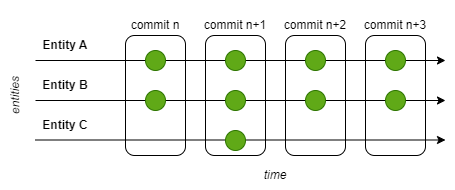
\includegraphics[scale=0.6]{dependencies.png}
\caption{Overview on updates of different entities}
\label{fig:dependencies}
\centering
\end{figure}

This type of entities, that consistently change together throughout development activities, are called logical dependencies or coupling. This concept was initially introduced by Gall et al. \cite{Gall:1998:DLC:850947.853338} and has numerous fields of application.

A problem with dependencies extracted from the versioning system is their potential to become excessively numerous. This often results from commits that contain numerous files, thereby generating thousands of dependencies from a single commit.
In our previous research, we examined several software systems and determined that commits involving a large number of files are frequently unrelated to code changes. \cite{enase19}.

Additionally, the reliability of co-changes is another problem; certain entities may only change together once throughout the entire versioning history, making them less reliable than entities that change together hundreds of times, for instance. Figure \ref{fig:dependencies} ilustrates this scenario.

Previous research uses two known metrics in order to solve this problems: \textit{support} and \textit{confidence}. Given a dependency where $A \rightarrow B$, the support metric measures the frequency of updates that two entities share within the versioning system. The confidence metric calculates the proportion of updates between two entities relative to the total updates of the antecedent (A) or consequent (B) entity \cite{DBLP:conf/issre/OlivaG15}, \cite{DBLP:journals/jss/AjienkaC17}, \cite{Zimmermann:2004:MVH:998675.999460}.


In our previous research, we focused on identifying metrics that enhance the reliability of dependencies extracted from the versioning system \cite{saci19}, \cite{enase19}. One of the metrics is the \textit{commit size metric}, which involves extracting dependencies from commits that do not exceed a specific commit size limit, thereby reducing the possibility of extracting an overly large number of dependencies. Additionally, we developed the strength metric, which serves as a refinement of the more known \textit{confidence metric} \cite{articlekeyclass23}.


The strength metric was developed to obtain a better reflection of the system and its values. For instance, when using the confidence metric, two entities that update together only once will have the highest possible score on the confidence metric, a result that is not desirable. On the other hand, entities that undergo hundreds of updates together, and even more updates with other entities, will receive a lower confidence metric score. Thus, the confidence metric will favor entities that update less and always together.

\begin{equation}
support (A \rightarrow B) = freq_{total\ commits} {(A \cup B)}
\end{equation}


\begin{equation}
confidence (A \rightarrow B) =\frac{support (A \rightarrow B) }{freq_{total\ commits}(A)}
\end{equation}

 The strength metric is calculated by multiplying the confidence metric value with a system factor, which is determined by the average number of updates for all entities in the system. In this way, a very high confidence score resulting from only a few updates will be adjusted downwards, while a low confidence score that is based on a big number of updates will be increased.

\begin{equation}
 system factor for (A \rightarrow B) =\frac{support (A \rightarrow B) }{system\ mean}
\end{equation}

\begin{equation}
 strength (A \rightarrow B) =\frac{support (A \rightarrow B) * 100}{freq_{total\ commits}(A)} * system\ factor
\end{equation}

The confidence metric score ranges from 0 to 1, with 1 representing the best value. On the other hand, the strength metric ranges from 0 to 100, where 100 represents the best possible score.

Co-changes that meet both the commit size metric threshold and the strength metric threshold are referred to as \textit{logical dependencies}.

\section{Related work}


Software clustering is the process of organizing software entities into groups(clusters) that correspond to the systems modules. There are numerous algorithms that can be used for software clustering such as hierarchical algorithms like Minimum Spanning Tree and Louvain that cluster software entities by their hierarchical relationships \cite{hicluster}, \cite{SoraSem13}. Partitioning algorithms, like k-means, that organize data into clusters by similarity \cite{5453745}. Density-based algorithms, such as DBSCAN, focus on areas of higher density to form clusters \cite{10.1145/304181.304187}, and many others \cite{Xu2015ACS}. 


Regarding the input data used by software clustering algorithms, some approaches rely solely on data derived from code dependencies (structural dependencies) to establish clusters \cite{SoraSem13}, \cite{891477}. The Bunch tool, developed by Mitchell and Mancoridis, utilizes source code analysis along with hill-climbing and genetic algorithms to create clusters from the code data \cite{Bunch1},\cite{Bunch2},\cite{Bunch3}.

Other approaches use lexical dependencies extracted from code comments \cite{5741257} or the name of the source files \cite{Anquetil1999RecoveringSA} \cite{Anquetil1998RecoveringSA}. 

A more recent approach involves using data from the system's historical changes in order to gain more knowledge about the system \cite{article-cochangem}. Co-changes have been used to analyze how the system's modularity evolves over time \cite{10.1145/3196398.3196409} or how co-changes impact the packaging restructuring \cite{clusters-cochange}.

Prajapati et al. used structural dependencies, lexical dependencies and co-changes from the versioning system to enhance system modularization \cite{clustering-ld-lexical}.

When it comes to evaluating the obatined clustering solutions,  if a reference solution exists, metrics can be applied to evaluate the similarity between the reference clustering solution and the obtained clusterings. One such metric is the MOJO distance, MOJO measures the minimum number of Move and Join operations required to transform one clustering solution into another \cite{mojo-tzerpos}. 


If no reference solution exists, then metrics that evaluate the cohesion of the clustering solution, based on the input graph, can be used. One such metric is the Modularization Quality (MQ) metric. As defined by Mitchell and Mancoridis \cite{mqmetric}, \cite{mqmetric2}, is extensively used to assess the results of clustering techniques. While it is primarily applied to clusters formed from structural dependencies \cite{Bunch1},\cite{Bunch2},\cite{Bunch3}, it can be used also for evaluating clusters derived from other types of dependencies \cite{clustering-ld-lexical}.


\section{Method}
\label{method}

\subsection{Dependencies extraction}
To obtain the logical dependencies for further use, we use a Python tool developed in our previous research \cite{articlekeyclass23}. This tool retrieves all necessary data from GitHub \cite{ApacheAntGitHub} using git commands and then processes it. 
The initial phase involves applying a commit size filter to exclude all commits that involve changes to more than 10 files. Following, the tool creates dependencies based on these commits, establishing a dependency link between each entity in a modified file and all entities in other files modified by the same commit. 

Next, the tool calculates the strength metric as described in chapter \ref{ld_def}. It then filters out any dependencies falling below the set strength metric threshold. For our experiments, we initiated with a strength metric threshold of 10, incrementing in steps of 10 up to 100 (the maximum value for the metric).Since the structural dependencies are oriented dependencies, we also export oriented logical dependencies. For entities A and B that update together, we calculate the strength metric for $A \rightarrow $B and $B \rightarrow $A, and export the dependency orientation that is above the set threshold. Finally, the results are exported in comma separated values format file (.csv). 

The above described workflow is illustrated in figure \ref{fig:extraction}.


\begin{figure}
\centering
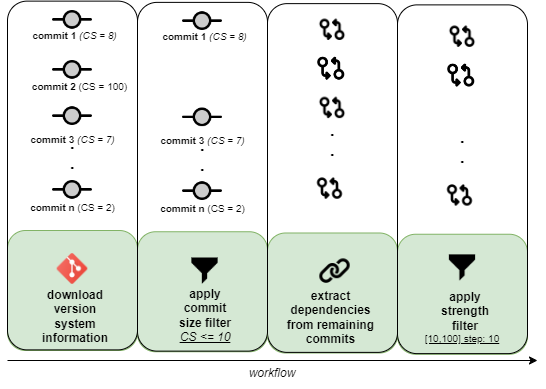
\includegraphics[width=\columnwidth]{dependencies-export.png}
\caption{Logical depenedencies extraction workflow}
\label{fig:extraction}
\centering
\end{figure}

\subsection{Louvain Clustering algorithm}

Following the generation of logical dependencies, we use them as input for software clustering. For this, a Python script was developed to extract both structural and logical dependencies from their respective files, forming a dependency matrix. This matrix is used as the input for the Louvain Clustering algorithm. 
Louvain Clustering is a community detection algorithm designed for finding clusters or communities in complex networks. The Louvain method involves a greedy algorithm that moves nodes between clusters to obtain clusters that are highly interconnected \cite{louvain_clustering}.

\subsection{Evaluation using MQ metric}
The resulting clustering solution is then evaluated using the Modularity Quality (MQ) metric . The MQ metric can vary between -1 and 1, where -1 means no cohesion within the modules, and 1 means no coupling between the modules \cite{mqmetric}.

To compare the clustering solutions and their MQ evaluation, we generated clustering solutions under three different scenarios. The first one by using only structural dependencies, the second one by using only logical dependencies, and the third one by using logical and structural dependencies to populate the dependency matrix that is further used in cluster generation. The workflow for the third scenario is illustrated in Figure \ref{fig:clustering-gen}.

\begin{figure}
\centering
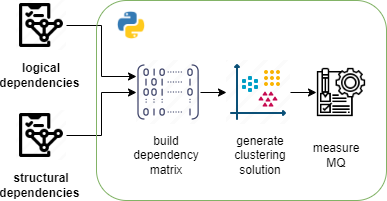
\includegraphics[width=\columnwidth]{clustering-generation.png}
\caption{Clustering solution creation process diagram}
\label{fig:clustering-gen}
\centering
\end{figure}


\section{Results}
\label{results}


The results of the scenarios mentioned in chapter \ref{method} are presented in tables \ref{tab:clustering-results1} and \ref{tab:clustering-results2}.
 In both tables, the first row shows the results from the clustering analysis relying solely on structural dependencies (scenario 1). We highlighted the results of structural dependencies in both tables for a more easy comparison with the results involving also logical dependencies.

Table \ref{tab:clustering-results1} presents the results when using only logical dependencies for software clustering. All rows, except the first one, represent the measurements obtained from logical dependencies extracted with varying strength thresholds.







\begin{table}[htbp]
  \centering
  \caption{Louvain clustering results for LD only}
  \label{tab:clustering-results1}
  \begin{tabular}{lc|c|c}
    \toprule
    \textbf{Dataset} & \textbf{Entities} & \textbf{Cluster} & \textbf{MQ } \\
    & \textbf{Count} & \textbf{count} &  \textbf{metric} \\
    \midrule
    SD only & 517 & 14 &  0.085  \\
    \midrule
LD  strength    10\%    &   320 &   75  &   0.383   \\
LD  strength    20\%    &   215 &   53  &   0.547   \\
LD  strength    30\%    &   174 &   44  &   0.558   \\
LD  strength    40\%    &   152 &   40  &   0.58    \\
LD  strength    50\%    &   138 &   35  &   0.604   \\
LD  strength    60\%    &   120 &   34  &   0.587   \\
LD  strength    70\%    &   106 &   32  &   0.577   \\
LD  strength    80\%    &   92  &   29  &   0.576   \\
LD  strength    90\%    &   79  &   24  &   0.606   \\
LD  strength    100\%   &   64  &   19  &   0.611   \\
    \bottomrule
  \end{tabular}
\end{table}


Table \ref{tab:clustering-results2} presents the results when using logical dependencies combined with structural dependencies for software clustering. All rows, except the first one, represent the measurements obtained from logical dependencies extracted with varying strength thresholds combined with structural dependencies extracted from static code analysis.

In both tables, the second column shows the total count of different entities forming dependencies in the system. The thirth column indicates the number of clusters obtained after injecting the dependencies to the Lovian algorithm. Lastly, the forth column indicates the MQ metric result computed for on the obtained clusters.

\begin{table}[htbp]
  \centering
  \caption{Louvain clustering results for LD and SD combined}
  \label{tab:clustering-results2}
  \begin{tabular}{lc|c|c}
    \toprule
    \textbf{Dataset} & \textbf{Entities} & \textbf{Cluster} & \textbf{MQ } \\
    & \textbf{Count} & \textbf{count} &  \textbf{metric} \\
    \midrule
    SD only & 517 & 14 &  0.085  \\
    \midrule
SD  LD  strength    10\%    &   517 &   15  &   0.087   \\
SD  LD  strength    20\%    &   517 &   13  &   0.071   \\
SD  LD  strength    30\%    &   517 &   13  &   0.071   \\
SD  LD  strength    40\%    &   517 &   13  &   0.071   \\
SD  LD  strength    50\%    &   517 &   13  &   0.071   \\
SD  LD  strength    60\%    &   517 &   13  &   0.071   \\
SD  LD  strength    70\%    &   517 &   13  &   0.071   \\
SD  LD  strength    80\%    &   517 &   13  &   0.071   \\
SD  LD  strength    90\%    &   517 &   13  &   0.071   \\
SD  LD  strength    100\%   &   517 &   13  &   0.072   \\

    \bottomrule
  \end{tabular}
\end{table}

Can be observed in Table \ref{tab:clustering-results1} that the MQ results for clustering solutions based solely on logical dependencies (LD) are not better than those based solely on structural dependencies (SD). In Column 2, it is noticeable that the total number of entities used decreases as the strength threshold increases. This trend is expected because stricter thresholds filter out more entities. But it is noticeable that this affects the overall quality of the clustering solutions obtained.

On the other hand, in Table \ref{tab:clustering-results2} can be observed that starting with the strength threshold of 20\% the MQ results for clustering solutions based on logical dependencies (LD) combined with structural dependencies (SD) are better than those based solely on structural dependencies (SD). 


\section{Discussion}
\label{discussion}

Based on the results from table \ref{tab:clustering-results2}, we can observe that the combined approach of structural dependencies and logical dependencies gives a Modularity Quality (MQ) metric of 0.071, which is an improvement over the 0.085 MQ metric obtained when considering only structural dependencies. 

We manualy compared two clustering solutions, the clustering solution obtained only from structural dependencies, in comparison to the clustering solution obtained from using both structural and logical dependencies, filtered with a threshold of 20\% for strength, in order to asses if the second solution is better or not.

The entities listed below are placed in different clusters: 

\begin{itemize}
    \item taskdefs.Available\$FileDir
    \item taskdefs.Concat
    \item taskdefs.Concat\$1
    \item taskdefs.Concat\$MultiReader
    \item taskdefs.Concat\$TextElement
    \item taskdefs.Javadoc\$AccessType
    \item util.WeakishReference
    \item util.WeakishReference\$HardReference
\end{itemize}


We will refer to the clusters resulted from the structural dependencies as \textit{Cluster A} and to those from logical and structural dependencies as \textit{Cluster B}.



In Cluster A, the Concat class and its inner classes (Concat\$1, Concat\$MultiReader, Concat\$TextElement) are placed together with conditions like Available, And, Or, IsTrue, Equals, IsReference, Contains.

On the other hand, Cluster B places them with classes associated with file manipulation and archive operations such as Ear, Jar, War, and Zip, as well as utility classes for file handling like FileUtils and JavaEnvUtils, and entities for zip file processing (ZipEntry, ZipFile).


The placement of the Concat class together with its inner classes in Cluster B can be motivated based on it's usage and purpose; according to the documentation : "This class contains the 'concat' task, used to concatenate a series of files into a single stream." \cite{ant_concat}. 
So, from our point of view, it is better placed in Cluster B, then in Cluster A.
Figure \ref{fig:cluster1} represents the connections that Concat has in the versioning and file system. Figure \ref{fig:clusterA} represents Cluster A connections and figure \ref{fig:clusterB} represents Cluster B connections.



\begin{figure}
\centering
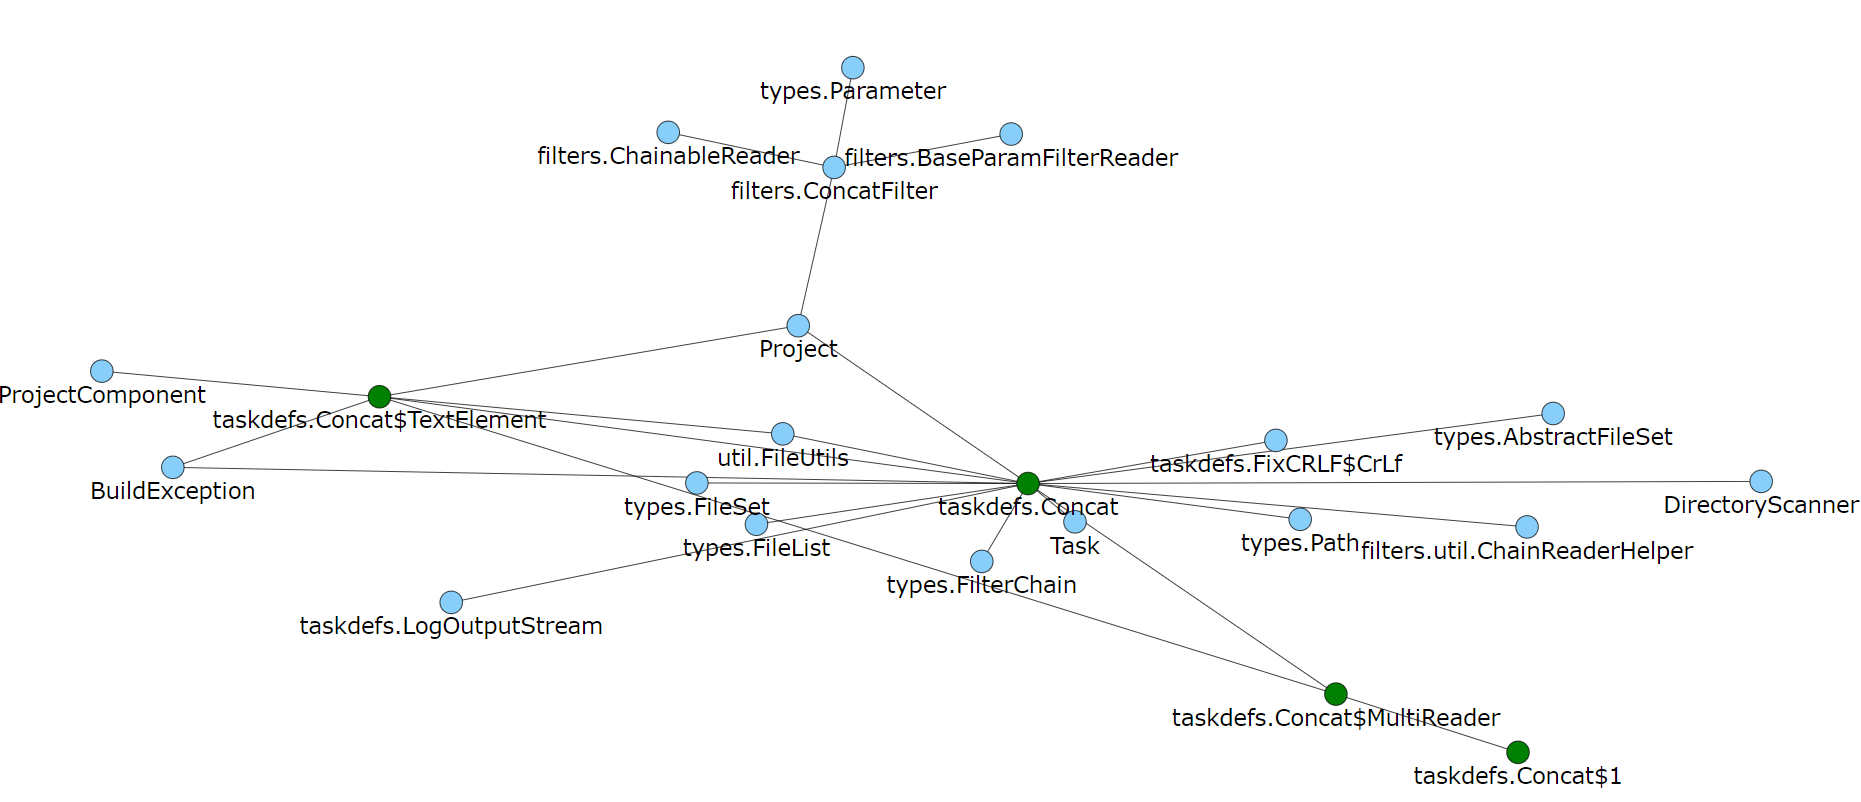
\includegraphics[width=\columnwidth]{dep.png}
\caption{Ant dependencies (LD and SD) of Concat class}
\label{fig:cluster1}
\centering
\end{figure}

\begin{figure}
\centering
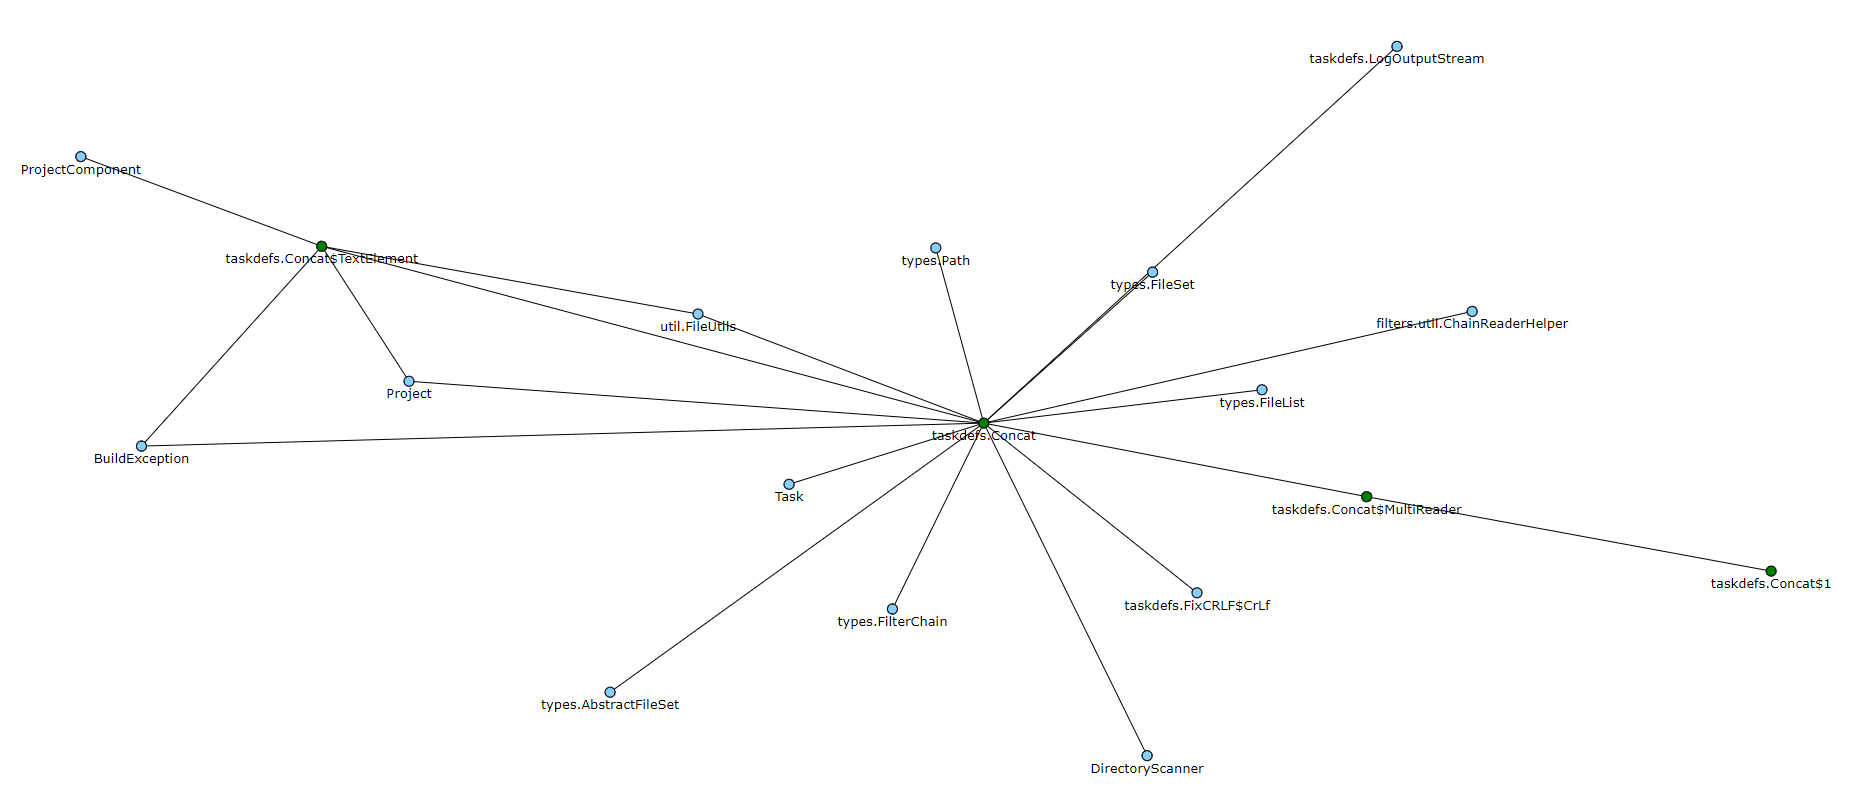
\includegraphics[width=\columnwidth]{cluster1.png}
\caption{Cluster A; cluster size: 25}
\label{fig:clusterA}
\centering
\end{figure}


\begin{figure}
\centering
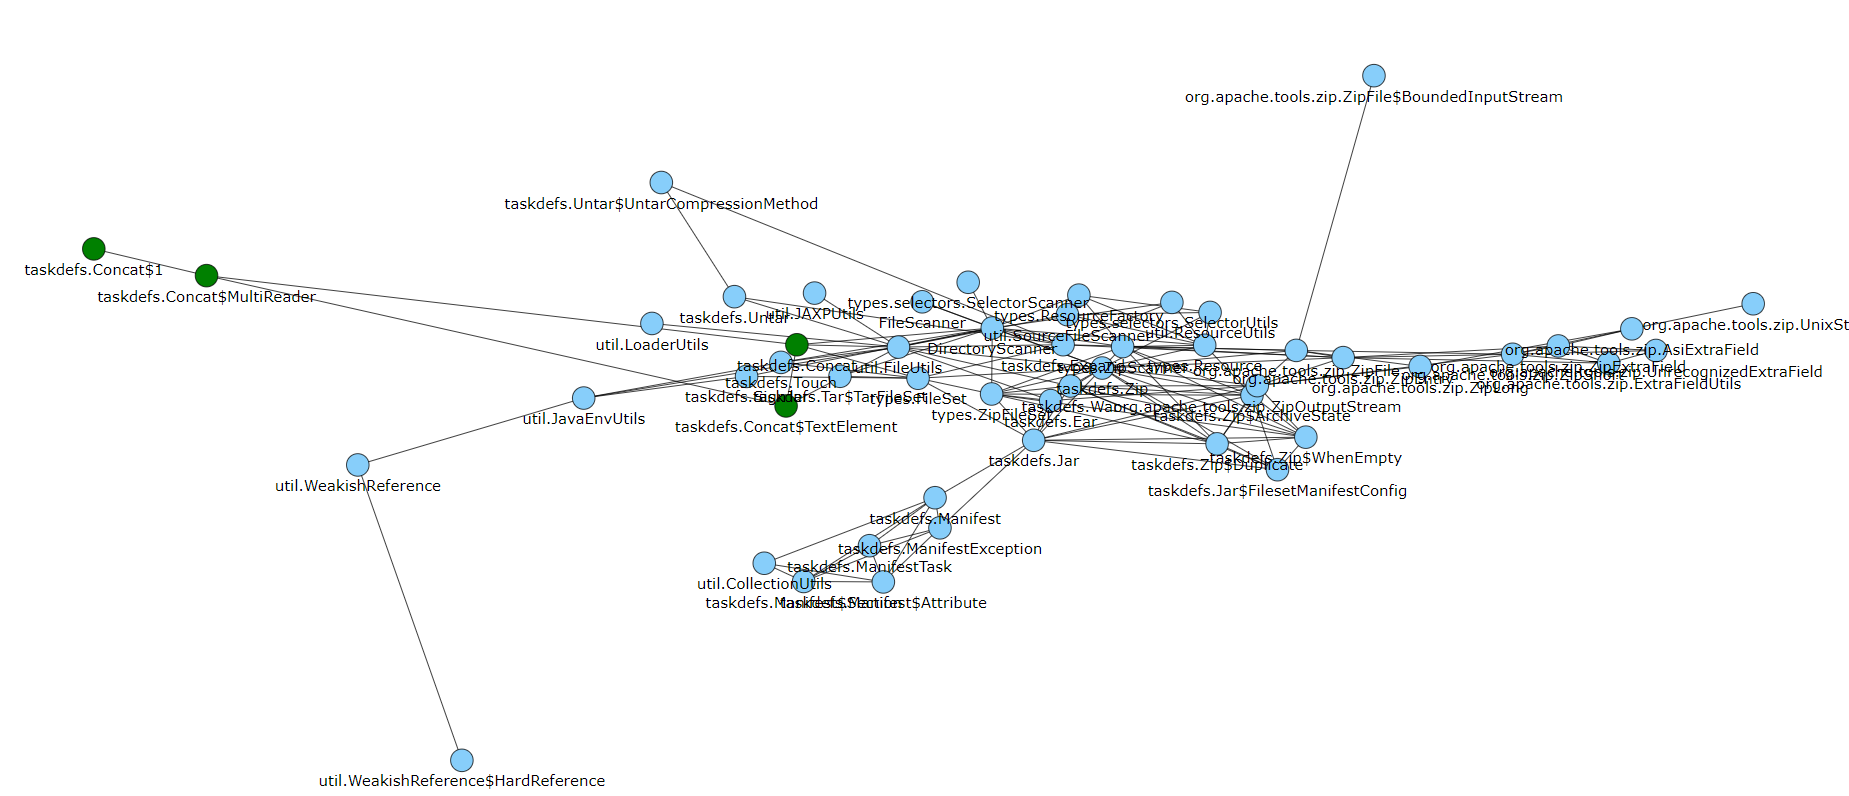
\includegraphics[width=\columnwidth]{cluster2.png}
\caption{Cluster B; cluster size: 52}
\label{fig:clusterB}
\centering
\end{figure}


The entity 'taskdefs.Available\$FileDir', in Cluster A, is clustered together with entities that are related to the build process (ProjectHelper, TaskAdapter, ComponentHelper), but do not have any relation to condition checks or file existence evaluations as does Available\$FileDir. 

Cluster B if formed by entities that are related to condition checking (And, Contains, Equals, Or, UpToDate), and also the outer class of 'taskdefs.Available\$FileDir',  'taskdefs.Available'. 

 The documentation description for 'taskdefs.Available' states: "Will set the given property if the requested resource is available at runtime. This task may also be used as a condition by the condition task."\cite{ant_concat}.
 This explains its association in Cluster B, which is centered around task definitions and conditions related to build processes.



\section{Conclusion and Future work}

Based the outcomes detailed in Chapter \ref{results} and the analysis in Chapter \ref{discussion}, it is clear that incorporating logical dependencies improves the quality of clustering solutions. For our forthcoming work, we intend to conduct further experiments across various projects to validate these findings. Additionally, we will try to create a reference clustering solution for these projects, based on their code and documentation. We will then evaluate the clustering results against the reference solution by utilizing the MOJO metric for comparison \cite{mojo-tzerpos}.


\bibliographystyle{IEEEtran}
\bibliography{logicaldepd}

\end{document}
